\section{Periodic table}
%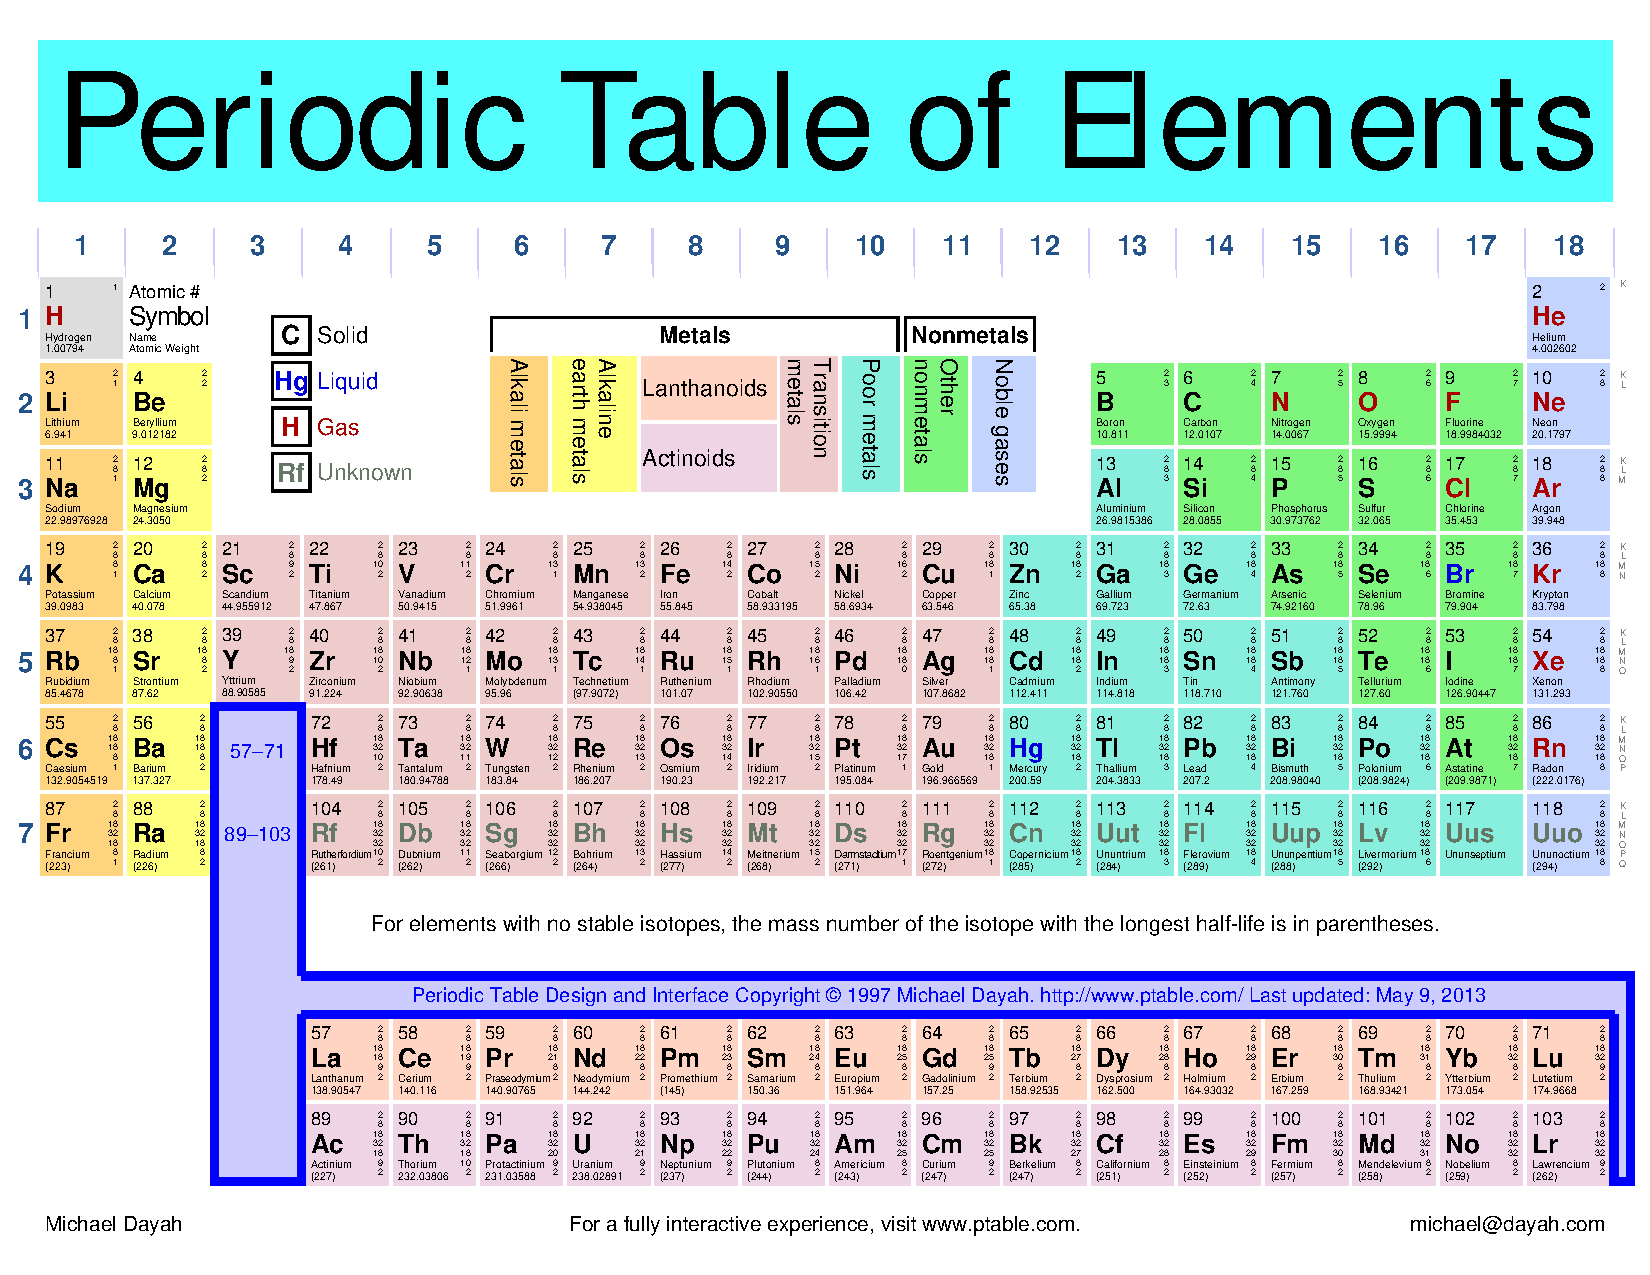
\includegraphics[width=\linewidth]{Periodic_Table.pdf}

\section{Seebeck coefficients}\label{app:Seebeck}
\begin{table}[htbp]
    \centering
    \begin{tabular}{lllll}
    Metal & S at \SI{0}{\degreeCelsius} (\si{\micro\volt\per\kelvin}) & S at \SI{27}{\degreeCelsius} (\si{\micro\volt\per\kelvin}) & $E_F$ (\si{\eV}) & x \\ \toprule
    Al   & -1.6    & -1.8   & 11.6 & 2.78    \\
    Au  & +1.79 & +1.94 & 5.5   & -1.48  \\
    Cu  & +1.70 & +1.84 & 7.0   & -1.79  \\
    K    &            &  -12.5 & 2.0   & 3.8      \\
    Li   & +14     &           & 4.7    & -9.7    \\
    Mg & -1.3    &           & 7.1    & 1.38     \\
    Na  &            & -5      & 3.1   & 2.2        \\
    Pd  & -9.00   & -9.99 &         &             \\
    Pt  & -4.45    & -5.28 &         &             \\ \bottomrule
    \end{tabular}
    \caption{Seebeck coefficients of selected materials. (Source: Kasap, Table 4.3)}
    \label{tab:app_seebeck}
\end{table}